\subsection{Line integrals}
\index{line integral}
Line integrals are easily computed by
converting the coordinates $x$, $y$ and $z$ into functions of $t$.
This has the effect of changing the measure as well.
For instance, $dx$ becomes $(dx/dt)\,dt$.
The following line integral problems are from
{\it Advanced Calculus, Fifth Edition} by Wilfred Kaplan.

\medskip
\noindent
Evaluate $\int y^2\,dx$ along the straight
line from $(0,0)$ to $(2,2)$.

\medskip
\verb$x=2t$

\verb$y=2t$

\verb$defint(y^2*d(x,t),t,0,1)$

$$8\over3$$

\medskip
\noindent
Evaluate $\int y\,dx$ along the straight line from
$(2,1)$ to $(1,2)$.

\medskip
\verb$x=2-t$

\verb$y=t+1$

\verb$defint(y*d(x),t,0,1)$

$$-{3\over2}$$

\medskip
\noindent
Evaluate $\int x\,dy$ along the straight line from
$(1,1)$ to $(2,1)$.

\medskip
\verb$x=t+1$

\verb$y=1$

\verb$defint(x*d(y),t,0,1)$

$$0$$

\medskip
\noindent
Evaluate $\int z\,dx+x\,dy+y\,dz$
along the path
$x=2t+1$, $y=t^2$, $z=1+t^3$, $0\le t\le 1$.

\medskip
\verb$x=2t+1$

\verb$y=t^2$

\verb$z=1+t^3$

\verb$f=z*d(x)+x*d(y)+y*d(z)$

\verb$defint(f,t,0,1)$

$$163\over30$$

\newpage

\noindent
If $g(t)$ is a function that parametrizes a curve from $a$ to $b$
then the arc length of the curve is
$$\int_a^b|g'(t)|\,dt$$
For example, let us measure the length of the following curve.

\medskip
\verb$xrange=(0,1)$

\verb$yrange=(0,1)$

\verb$draw(x^2)$

\begin{center}
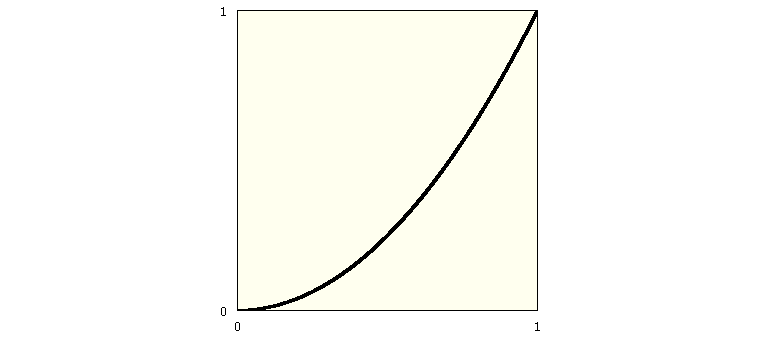
\includegraphics[scale=0.4]{arc.png}
\end{center}

\medskip
\noindent
For the parametrization
$$g(t)=(t,t^2),\qquad0\le t\le 1$$
the Eigenmath solution is

\medskip
\verb$g=(t,t^2)$

\verb$defint(abs(d(g,t)),t,0,1)$

$$\hbox{$1\over4$}\log(2+5^{1/2})+\hbox{$1\over2$}5^{1/2}$$

\verb$float$

$$1.47894$$

\medskip
\noindent
As we would expect, the result is longer that the diagonal $\sqrt2$.

